\section{Introduction}
\label{sec:intro}

Flow Matching \citep{lipman2023flow, albergo2023building, liu2023flow} has emerged as a state-of-the-art paradigm for continuous-time generative modelling, offering simulation-free training and straightforward extension to Riemannian manifolds \citep{chen2024flow, mathieu2020riemannian}. Interest has recently grown in applying these methods to complex-valued physical signals $z = x + iy = A e^{i\theta} \in \mathbb{C}$, such as Magnetic Resonance Imaging (MRI) or Audio Spectrograms, where the signal phase $\theta$ encodes critical structural and physical properties. 

However, existing frameworks almost universally force complex signals into a naive Euclidean embedding: the data is treated as a two-channel flat Cartesian vector $(\mathrm{Re}(z), \mathrm{Im}(z)) \in \mathbb{R}^2$. As illustrated in Figure~\ref{fig:teaser_flow}, the plane itself is perfectly well behaved; what suffers is the probability path drawn on it. Straight Euclidean probability paths $z(t) = (1-t)z_0 + t z_1$ obey the triangle inequality, which pulls intermediate states below the amplitude of either endpoint, and arbitrarily close to the origin when the phases are near-antipodal. Furthermore, the phase of a Cartesian path can turn arbitrarily fast when the endpoints are close to antipodal. The Cartesian target $z_1 - z_0$ is itself bounded whenever the endpoints are; what is unbounded is the rate at which the path turns, and that is what a coarse integrator has to resolve.

\begin{figure}[t]
    \centering
    \begin{subfigure}[b]{0.48\textwidth}
        \centering
        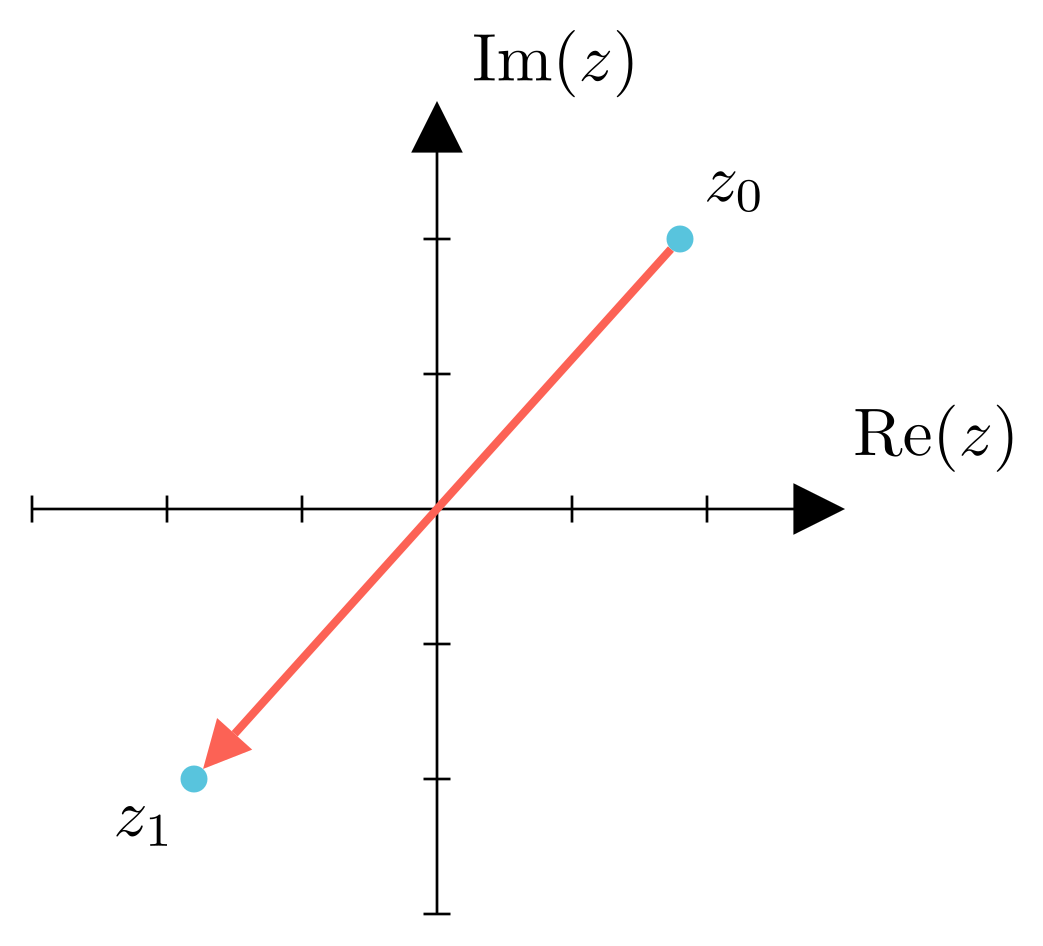
\includegraphics[height=2.9cm, keepaspectratio]{figures/EuclideanFlow_cropped.png}
        \caption{Standard Euclidean Flow ($\mathbb{R}^2$)}
        \label{fig:flow_euclidean}
    \end{subfigure}
    \hfill
    \begin{subfigure}[b]{0.48\textwidth}
        \centering
        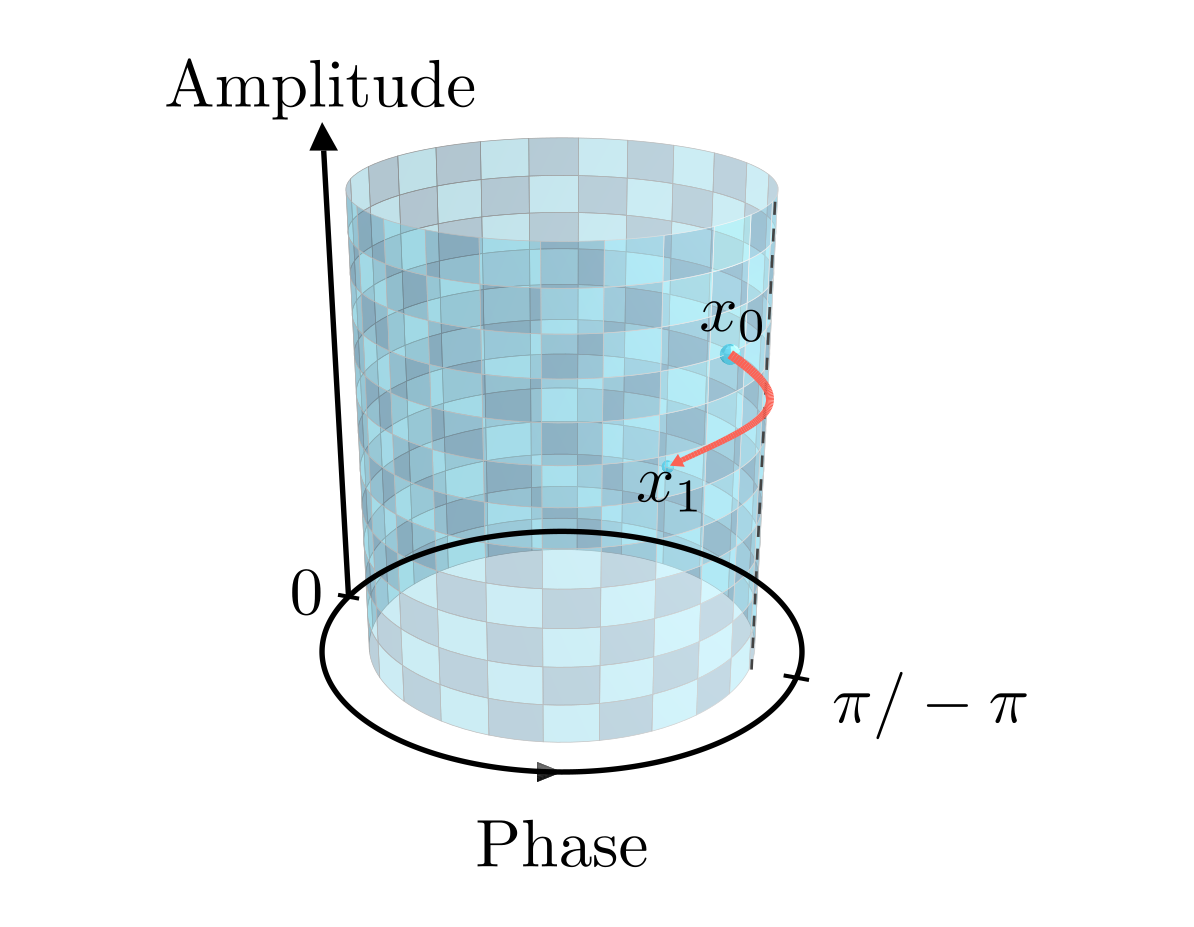
\includegraphics[height=2.9cm, keepaspectratio]{figures/CylindricalFlow_cropped.png}
        \caption{Cylindrical Flow Matching (Ours)}
        \label{fig:flow_cylindrical}
    \end{subfigure}
    \caption{\textbf{Geometric mismatch in complex-valued generative flows.} \textbf{(a)} In the Euclidean complex plane $(\mathrm{Re}(z), \mathrm{Im}(z))$, linear probability trajectories pass close to the origin, inducing severe midpoint amplitude attenuation ($|z_{1/2}| \ll \frac{1}{2}(|z_0| + |z_1|)$). \textbf{(b)} Cylindrical Flow Matching works in amplitude--phase coordinates on $(0, \infty) \times S^1$ under the decoupled product metric, transporting phase along the minimal circular geodesic while preserving amplitude.}
    \label{fig:teaser_flow}
    \vspace{-2mm}
\end{figure}

Prior work in representation learning and abstract feature alignment has proposed decoupled metrics on cylindrical or polar product manifolds to alleviate these issues \citep{chen2026dpfm, wang2026disrfm}. However, attempting to scale these Riemannian formulations to raw, high-dimensional complex wavefields introduces entirely new failure modes associated with spatial coherence and empirical Optimal Transport (OT). 

In this paper, we conduct an empirical analysis of Euclidean versus Cylindrical Flow Matching for complex-valued synthesis across three diverse domains: synthetic complex fields with known ground truth, speech audio STFT spectrograms, and raw complex fastMRI knee wavefields. We define \textbf{Cylindrical Flow Matching (CyFM)} on the product manifold $\mathcal{M} = [0, \infty) \times S^1$ with a decoupled product metric, whose target angular velocity is bounded by construction ($|u_\theta| \le \pi$), and measure on exact analytical probability paths what the Cartesian alternative costs. We couple noise and data by exact minibatch OT computed jointly over whole fields in the cylindrical metric, and find that although its transport-cost reduction collapses as the field dimension grows, its benefit to few-step generation persists. Finally, we expose the ``Factorised Coupling Trap'', a common but flawed countermeasure where transport plans are factored per-dimension or per-patch, which we show destroys the joint distribution.

\textbf{Contributions.}
\begin{itemize}
    \item \textbf{Bridge geometry.} We measure, on exact probability paths, how fast the phase has to turn. The Cartesian bridge has a heavy tail with power-law index $\approx 1$, which we derive in closed form for equal amplitudes: under independent coupling, nearly half of its paths exceed an angular speed of $\pi$, the bound the cylindrical target never crosses at any coupling.
    \item \textbf{Few-step generation across domains.} Across synthetic fields ($16\times16$ to $64\times64$), real speech STFT ($64\times64$), and raw complex fastMRI knee wavefields ($64\times64$), CyFM with the joint coupling reaches a lower error than the best Cartesian baseline at every $k \le 8$ integration steps, with all five seeds separated and no distillation, achieving up to $1.8\times$--$3.0\times$ error reduction at $k=1$. Run to convergence, we detect no significant difference between them.
    \item \textbf{Joint OT at field scale.} We couple noise and data by exact minibatch OT over whole fields in the cylindrical metric. Its saving in transport cost shrinks as the field grows, from 86\% on scalar pairs to 3\% for $64\times64$ fields (batch 64). The few-step error of the cylindrical model still drops by 3--60\% at every resolution we evaluated.
    \item \textbf{The factorised coupling trap.} Factorising that coupling per coordinate (amplitude/phase) or per patch is the obvious way around the cost of OT in high dimension. It quietly destroys the target instead. The marginals survive intact, the dependence between them does not, and structural coherence across patch seams goes with it.
\end{itemize}
